% Anexo: Manual de Usuario para la Aplicación Neural Analytics
\chapter*{Anexo III: Manual de Usuario de la Aplicación Neural Analytics}
\addcontentsline{toc}{chapter}{Anexo III: Manual de Usuario de la Aplicación Neural Analytics}

Este anexo es un manual detallado para el uso de la aplicación gráfica de Neural Analytics. Aquí se explica cada pantalla, el flujo de trabajo y las acciones que debe realizar el usuario en cada momento, con el objetivo de que cualquier persona pueda utilizar la aplicación de principio a fin.

\section*{1. Antes de empezar}
\begin{itemize}
    \item Asegúrese de tener el dispositivo BrainBit cargado y listo.
    \item Compruebe que la aplicación Neural Analytics está instalada en su ordenador.
    \item Tenga a mano el archivo de modelo de inferencia (si es necesario cargarlo manualmente).
\end{itemize}

\section*{2. Pantalla de carga}
Al abrir la aplicación, verá una pantalla de bienvenida con el nombre del sistema y una animación de carga. Espere unos segundos hasta que la aplicación termine de prepararse.

\begin{figure}[h!]
    \centering
    \includegraphics[width=0.7\textwidth]{assets/screenshots/inference/loading_app.png}
    \caption{Pantalla de carga inicial de la aplicación.}
\end{figure}

\section*{3. Pantalla de bienvenida}
Cuando la aplicación esté lista, aparecerá una pantalla que le pedirá encender la diadema EEG y colocársela correctamente. Siga la instrucción y espere a que el sistema lo detecte.

\begin{figure}[h!]
    \centering
    \includegraphics[width=0.7\textwidth]{assets/screenshots/inference/welcome_user.png}
    \caption{Pantalla de bienvenida e instrucciones para colocarse la diadema.}
\end{figure}

\section*{4. Calibración de electrodos}
Tras colocarse la diadema, la aplicación le guiará por una pantalla de calibración. Aquí podrá ver el estado de cada electrodo (T3, T4, O1, O2) mediante indicadores visuales (colores o iconos). Si algún electrodo aparece en rojo o con un símbolo de error, ajuste su posición hasta que todos estén en verde o con el símbolo de correcto.

\begin{figure}[h!]
    \centering
    \includegraphics[width=0.7\textwidth]{assets/screenshots/inference/headset_calibration.png}
    \caption{Pantalla de calibración de electrodos.}
\end{figure}

\section*{5. Pantalla principal de inferencia}
Una vez calibrados los electrodos, accederá a la pantalla principal. Aquí podrá:
\begin{itemize}
    \item Ver en tiempo real las señales recogidas por cada electrodo, representadas en gráficas.
    \item Consultar el estado del sistema y el color de "pensamiento" detectado (por ejemplo, rojo o verde).
\end{itemize}

\begin{figure}[h!]
    \centering
    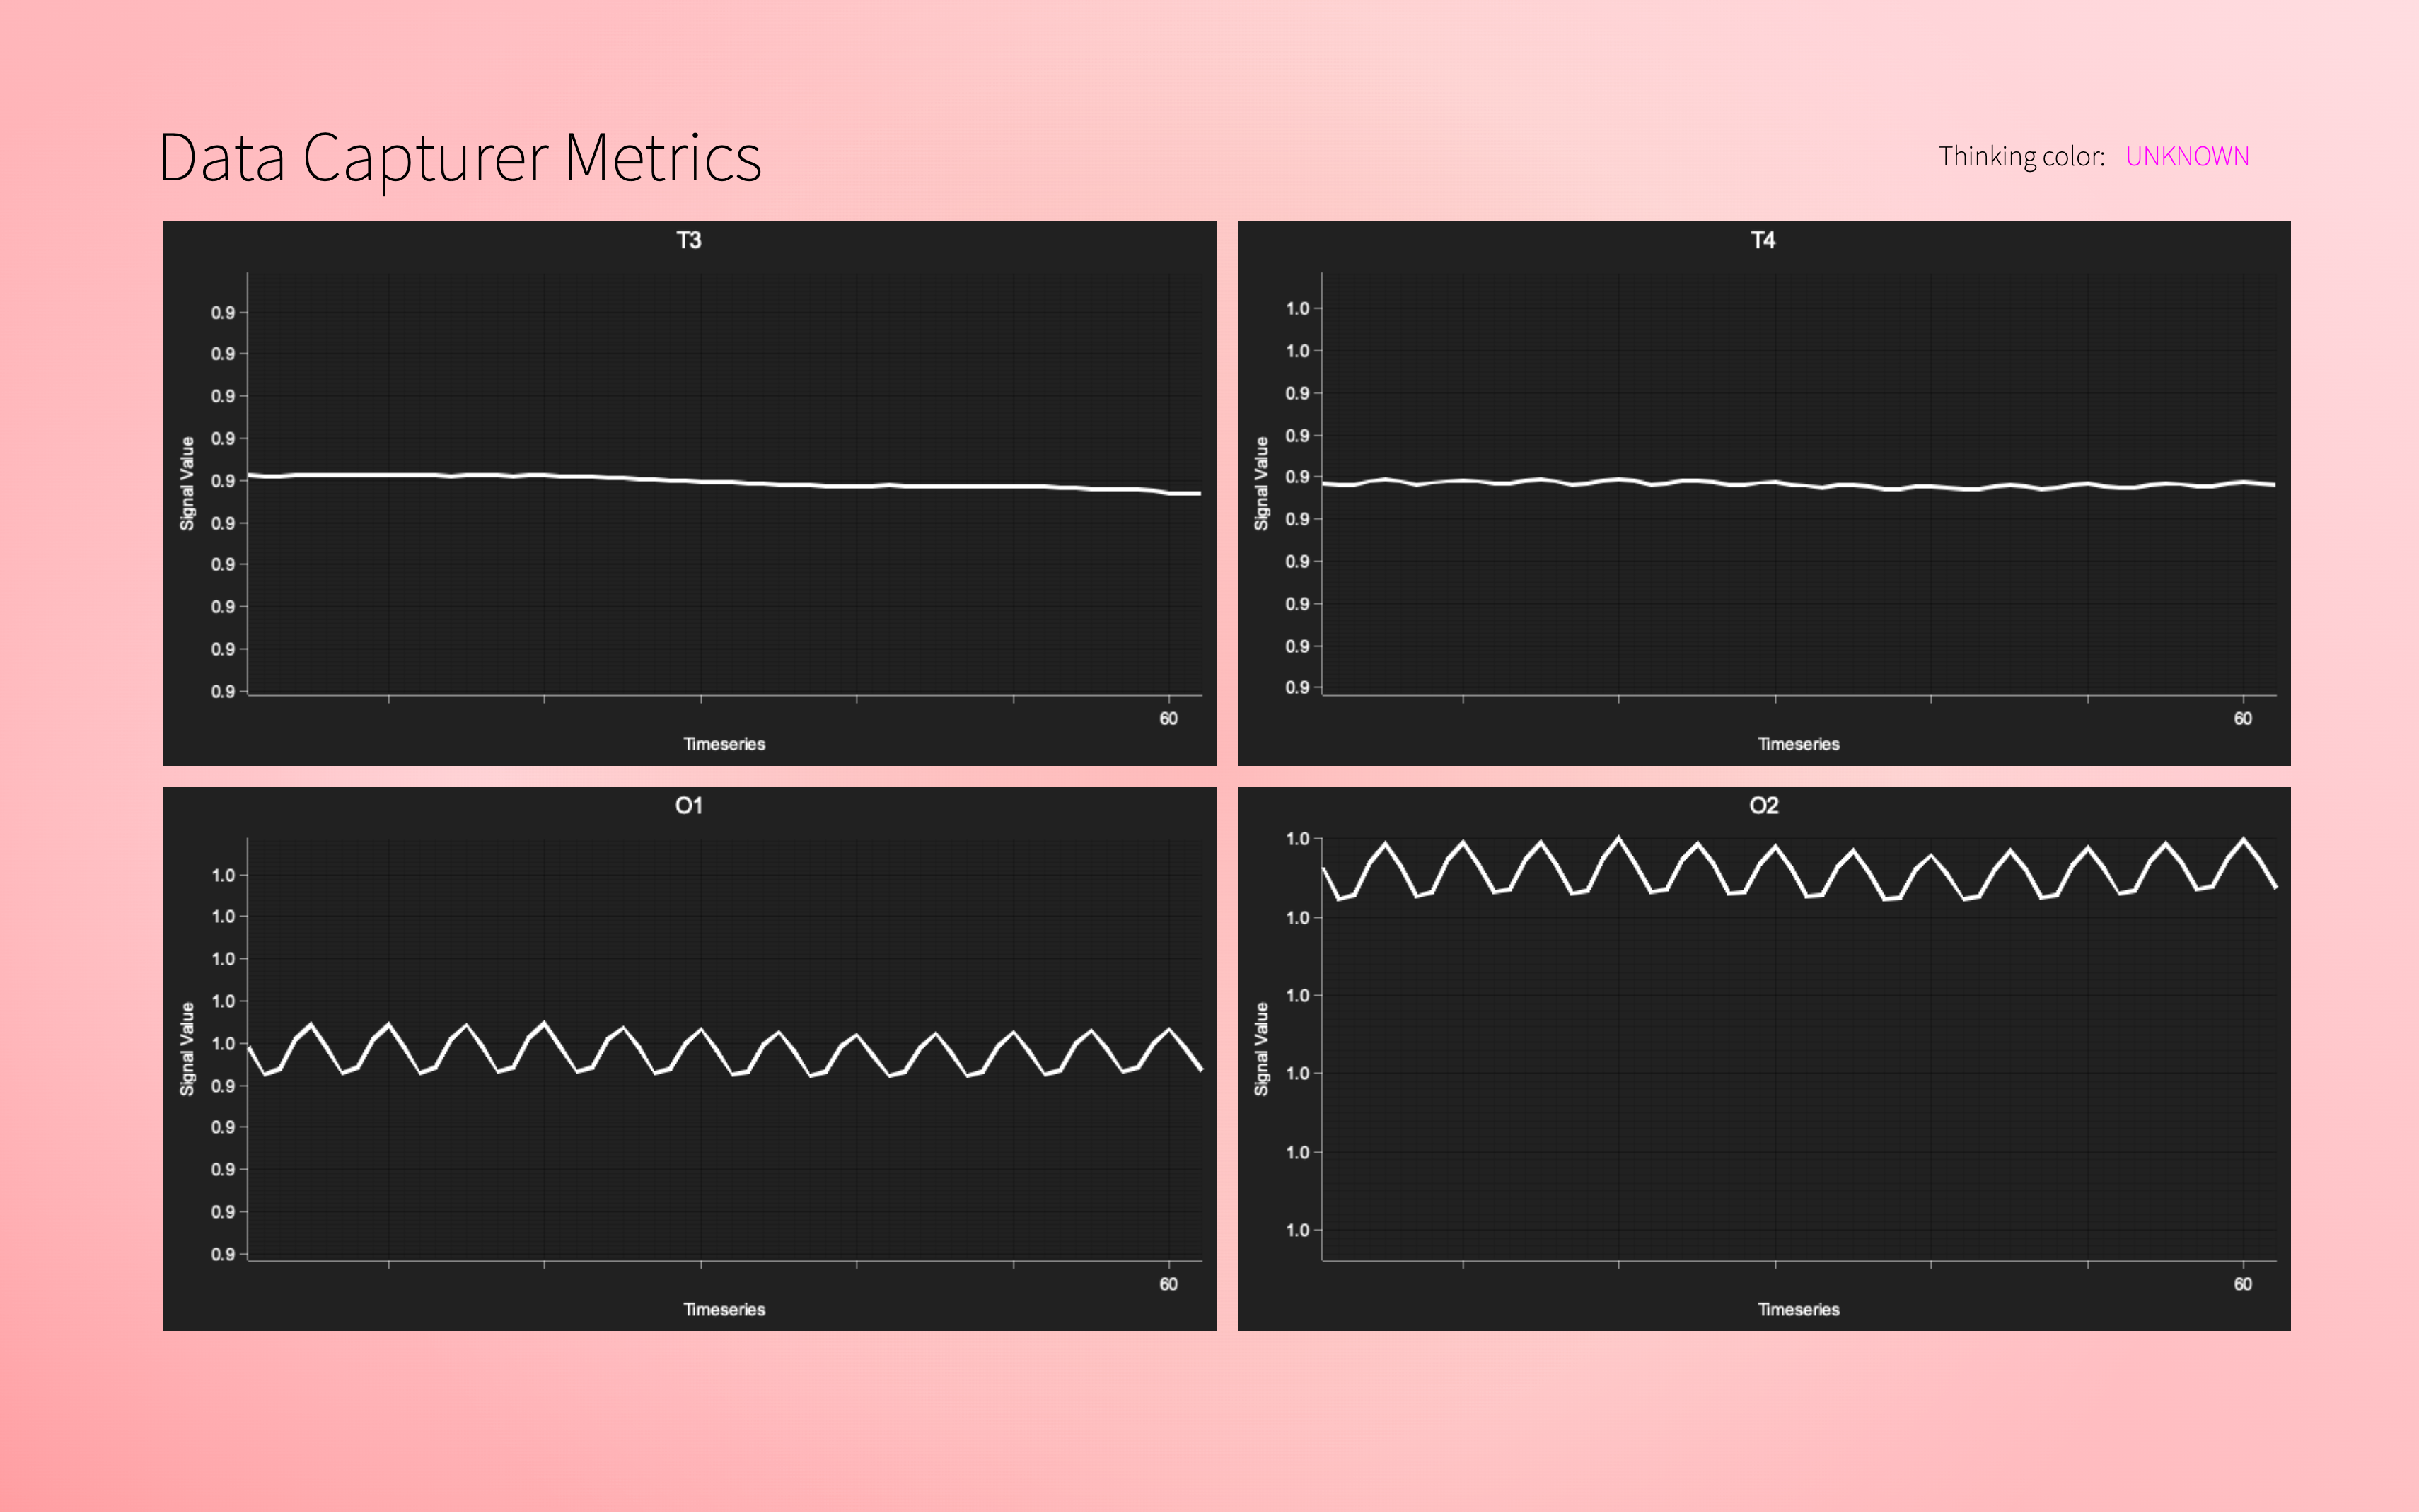
\includegraphics[width=0.8\textwidth]{assets/screenshots/inference/main_window.png}
    \caption{Pantalla principal de la aplicación de inferencia.}
\end{figure}

\section*{6. Mensajes y estados de la aplicación}
\begin{itemize}
    \item Si algún electrodo pierde contacto, la aplicación lo indicará y le pedirá ajustarlo.
    \item Si la señal es débil o hay interferencias, aparecerá un aviso. Siga las recomendaciones en pantalla.
    \item Si todo está correcto, los indicadores estarán en verde y podrá continuar.
    \item En caso de error grave, reinicie la aplicación y repita el proceso desde el inicio.
\end{itemize}

\section*{7. Consejos prácticos}
\begin{itemize}
    \item Coloque la diadema de forma cómoda y estable, evitando movimientos bruscos durante la sesión.
    \item Si ve que al usuario le aprieta mucho la banda para que sea conductiva, pruebe a mojar la cabeza del usuario con agua o gel para mejorar la conductividad.
    \item Si tiene dudas, consulte este manual o pida ayuda al responsable.
\end{itemize}
